\chapter{Methodology}\label{method}

\section{Flow of the project}

Figure \ref{fig:flowproj} shows the flowchart of the development of the entire project. The project started with literature review to understand the basic concepts for FRBs such as their properties and progenitor theories, as well as theories regarding available FRB detection methods and pipelines used on various radio telescope. Then, I proceeded to explore pulsar and transient analysis programs such as SIGPROC and PRESTO in order to understand basic processes in radio telescope data processing. I also gathered FRB data from radio telescopes used in previous researches, as well as develop a code to generate fake FRB data. Next, I learned and explored BEAR to understand more on the processes regarding FRB data analysis, as well as tested it with the available data. With that, I then developed the independent FRB detection program, and tested it out similarly. After that, the program's performance was analyzed and compared with BEAR, and finally, GPU implementation was tested out, specifically for dedispersion.

% The project starts with understanding the basic concepts for FRBs such as their properties and progenitor theories. Then, I continued to explore the available FRB detection methods and pipelines used at various radio telescopes. Following that, I wrote the literature review as required regarding both topics. I then proceeded to obtain FRB data from previous researches e.g. from the Parkes Telescope, as well as writing a code which generates FRB data to test detection programs with. Next, I tried out various pulsar and FRB programs such as SIGPROC, PRESTO, and BEAR, as well as understanding the underlying processes involved. From this, I then produced the FRB detection program (PoLaR BEAR) and proceeded to test with the FRB data available. Lastly, I tested out 

\begin{figure}[h]
    \vspace{1em}
    \centering
    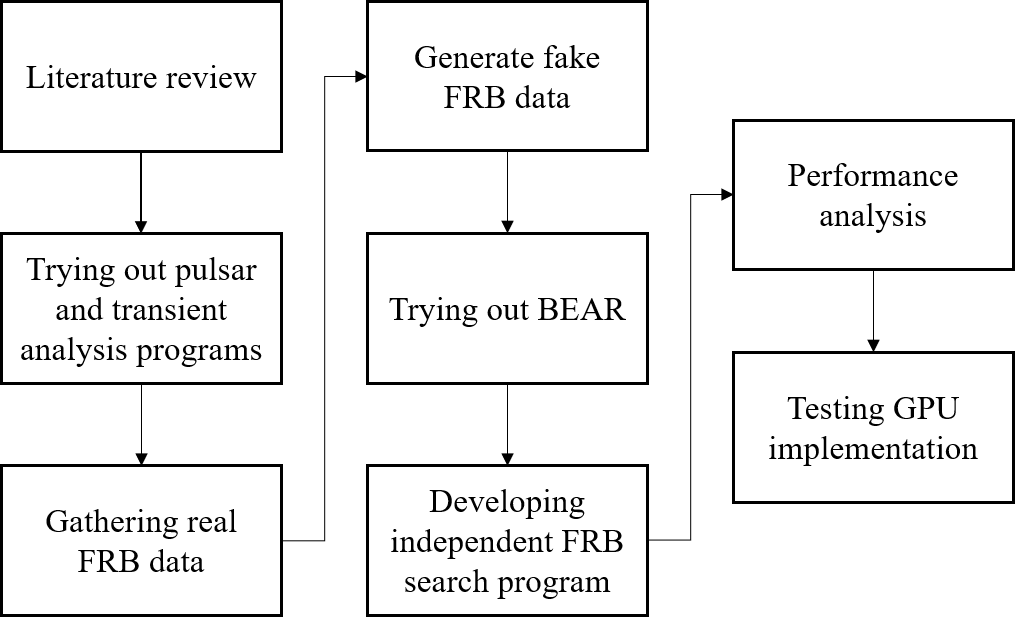
\includegraphics[width=0.9\textwidth]{Images/flowproj.png}
    \vspace{0.5em}
    \caption{Flowchart of the development of the project.}
    \label{fig:flowproj}
\end{figure}

\section{Introduction to PoLaR BEAR}

This independent FRB searching program is developed based on the Burst Emission Automatic Roger (BEAR), as demonstrated in \citeNP{Men2019}, which is an FRB searching pipeline mainly written in C++ (with some Fortran and Python), and utilizes many pulser/radio transients searching programs such as \texttt{SIGPROC}, \texttt{PRESTO}, \texttt{CFITSIO}, \texttt{PSRCAT}, \texttt{PSRCHIVE}, \texttt{TEMPO}, and \texttt{TransientX}. This project uses Python due to:
\begin{itemize}
    \item Relatively modern language;
    \item Easily understood and modified by beginners and advanced users;
    \item Indexing style of operation for functions rather than performing loops; and
    \item Ability to utilize and handle multidimensional arrays.
\end{itemize}
This program will also be standalone, requiring only a few general Python packages. This program will be referred to as the `PythOn LAnguage Radio Burst Emission Automatic Roger' or PoLaR BEAR. Shown in Figure \ref{fig:flowbear} is the block diagram/flowchart for the procedures in PoLaR BEAR. The following sections will explain each procedure in detail.

\begin{figure}[h]
    \vspace{1em}
    \centering
    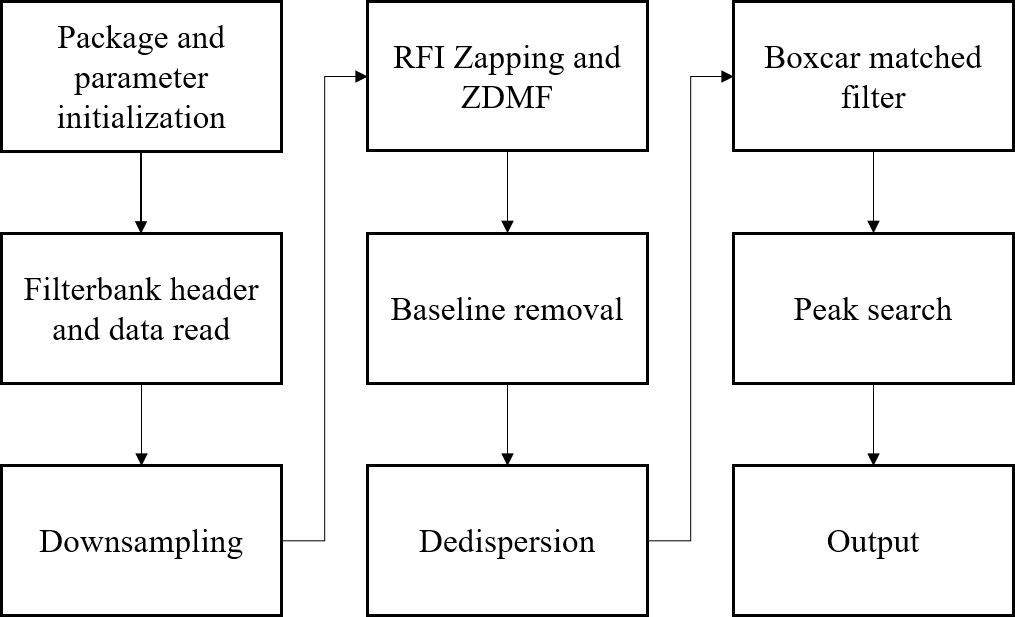
\includegraphics[width=0.9\textwidth]{Images/flowbear.png}
    \vspace{0.5em}
    \caption{Block diagram for procedures in PoLaR BEAR.}
    \label{fig:flowbear}
\end{figure}

\section{Initialization}

The first section of the program involves the initialization of the required packages:
\begin{enumerate}
    \item \texttt{Numpy}: Handles mathematical functions and multidimensional single data type arrays,
    \item \texttt{Struct} and \texttt{Bitarray}: Handles and operates on binary data types,
    \item \texttt{Matplotlib}: Plotting of data, analysis output, etc.
    \item \texttt{Tabulate}: Formatting the output in table form.
\end{enumerate}
Analysis parameters are also defined here. 

Then, the data is read. The type of radio telescope data that are used are called filterbanks, which are binary data files \cite{Lorimersigproc}. These files consists of two parts; header and data. The header stores the parameters of the data e.g. telescope ID, machine ID, source name, the sky coordinates the telescope is pointing towards, start time of the data, sampling time, frequency channels, polarization channels, and the number of bits of the data. The data then consists of correlated and integrated voltage data from the radio telescope's receiver, arranged in time, polarization channels and frequency channels. The program reads the header to a Python dictionary, and the data to a bytearray object. To reduce memory usage, the data is slice using bitarray indexing based on the set start and end times. Finally, the data is converted into a 64-bit \texttt{Numpy} float 2-D array.

\section{Pre-analysis}

After the data is extracted, the next part is the pre-analysis i.e. the preparation of the data before further analysis. First, the program performs downsampling where the data is summed every certain number of samples to reduce the time resolution of the data. Here \texttt{numpy.add.reduceat} is utilized i.e. performing local addition with specified slices. This is done also to reduce the size of the data as well the computation cost. 

Then, the program performs RFI mitigation. Here two methods are used; zapping RFI and the zero-DM matched filtering or ZDMF for short. Zapping RFI is to remove the data from frequency channels which are contaminated with RFI, which is a very common measure in radio astronomy e.g. signals at 1.55 GHz due to RFI from satellite communication \cite{Zhang2021}. Then, ZDMF is performed, where narrow band RFI with no dispersive measure is removed \cite{Men2019}. The program starts by estimating the zero-DM time series by summing the data over all the temporal domain, denoted as $\mathbf{s}_{\text{DM=0}}$. Then, the residual of fitting the zero-DM waveform to every channel is reduced into
\begin{equation}
    \chi^2 = (\mathbf{s}_i - \alpha_i\mathbf{s}_{\text{dm=0}} - \beta_i)^2
\end{equation}
where $\alpha_i$ is the scale factor given as 
\begin{equation}
    \alpha_i = \frac{\mathbf{s}_{\text{dm=0}}\cdot\mathbf{s}_i - \frac{1}{N} \sum \mathbf{s}_i \sum \mathbf{s}_{\text{dm=0}}}{\mathbf{s}_{\text{dm=0}}\cdot\mathbf{s}_{\text{dm=0}} - \frac{1}{N} \sum \mathbf{s}_{\text{dm=0}} \sum \mathbf{s}_{\text{dm=0}}}
\end{equation}
and $\beta_i$ is the baseline (not considered here as it does not affect pulse detection). Therefore, the RFI is removed from the data by obtaining the new time series at the $i$-th channel using
\begin{equation}
    \mathbf{s}_i' = \mathbf{s}_i - \alpha_i \mathbf{s}_{\text{dm=0}}
\end{equation}
Shown in Figure \ref{fig:zdmf} is an example of the usage of ZDMF on generated FRB data with a narrow-band RFI over a short duration.
\begin{figure}
    \centering
    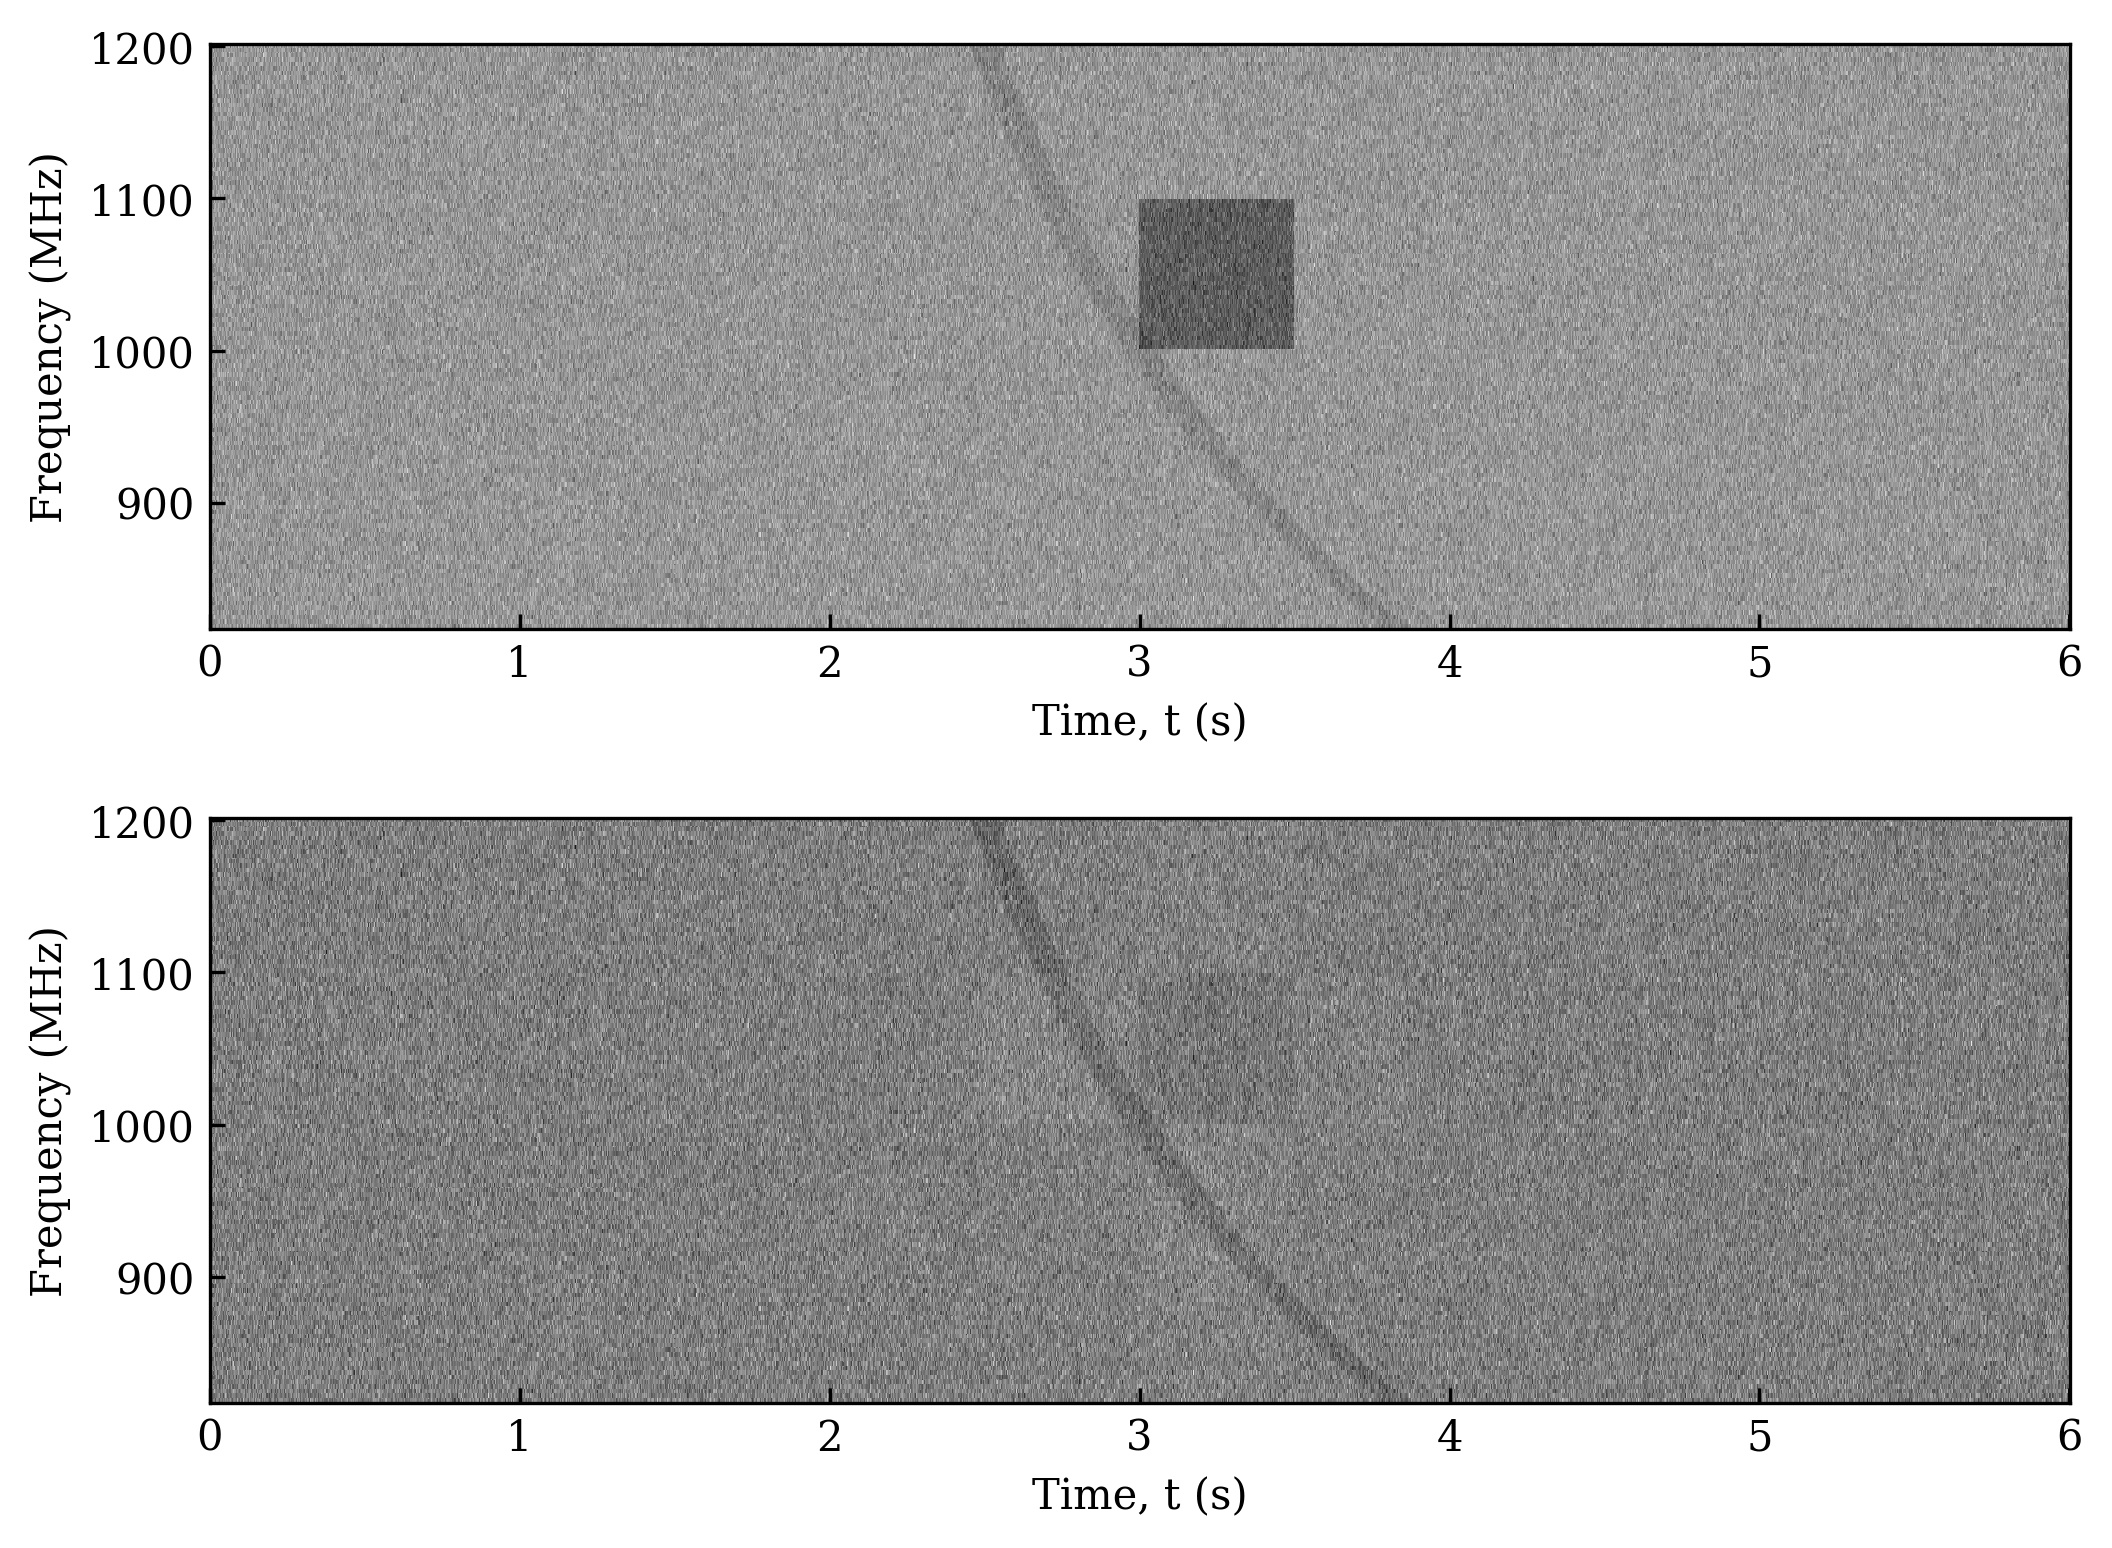
\includegraphics[width=\textwidth]{Graphs/ZDMF.jpeg}
    \caption[Application of zero-DM matched filter]{Frequency spectrum of generated FRB data at $\text{DM}=400\cmp$ with a narrow-band RFI over a short duration, before (upper) and after zero-DM matched filter (lower).}
    \label{fig:zdmf}
\end{figure}

The final step before the analysis is to perform baseline removal i.e. calibrating the data in every channel to have equal averages. For frequency channels with non-zero mean, the new time series at the $i$-th channel is
\begin{equation}
    \mathbf{s}_i' = \mathbf{s}_i - \bar{\mathbf{s}}_i
\end{equation}

\section{Analysis}

After the pre-analysis is complete, the program continues the analysis by performing three operations; dedispersion, boxcar matched filter, and pulse search. Dedispersion is performed to remove the time delay due to the cold-plasma dispersion, so that the pulse occur at the same time in all frequency channels, maximizing the SNR of the FRB. This is done by calculating the delay for every channel using Equation \ref{eq:dmdelay}, and then shifting the data in the time axis based on that delay, in this case using \texttt{numpy.roll}. Figure \ref{fig:dedisp} shows an example of dedispersion performed on FRB data. Summing over all the frequency channels gives the pulse profile of the FRB. For an FRB data with unknown DM, the data is dedispersed at many trial DMs, producing a set of profiles, which is referred to as 1-D dedispersed time series. 

\begin{figure}
    \centering
        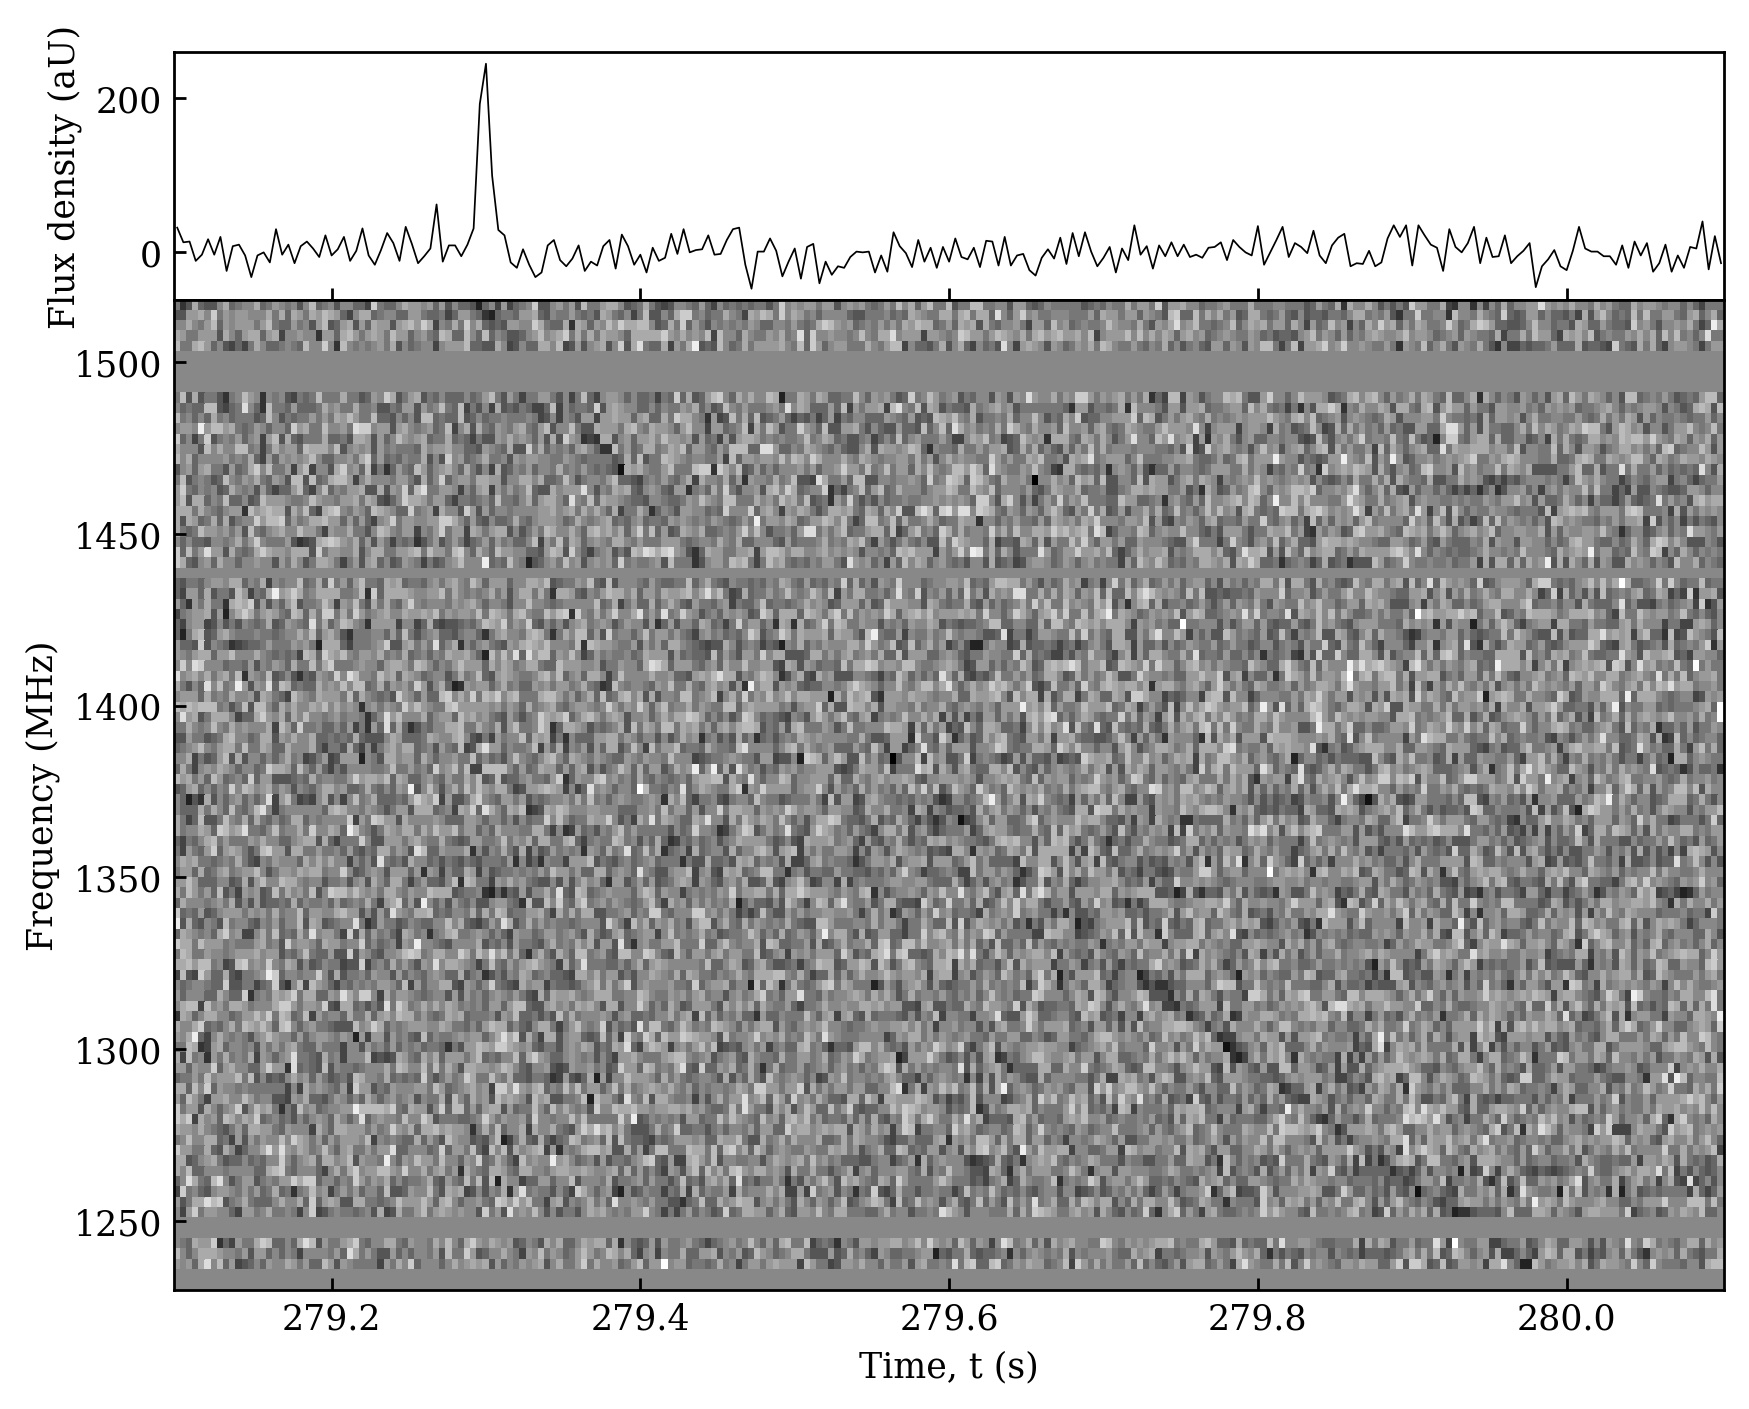
\includegraphics[width=0.8\textwidth]{Images/FRB010621disp.jpg}
        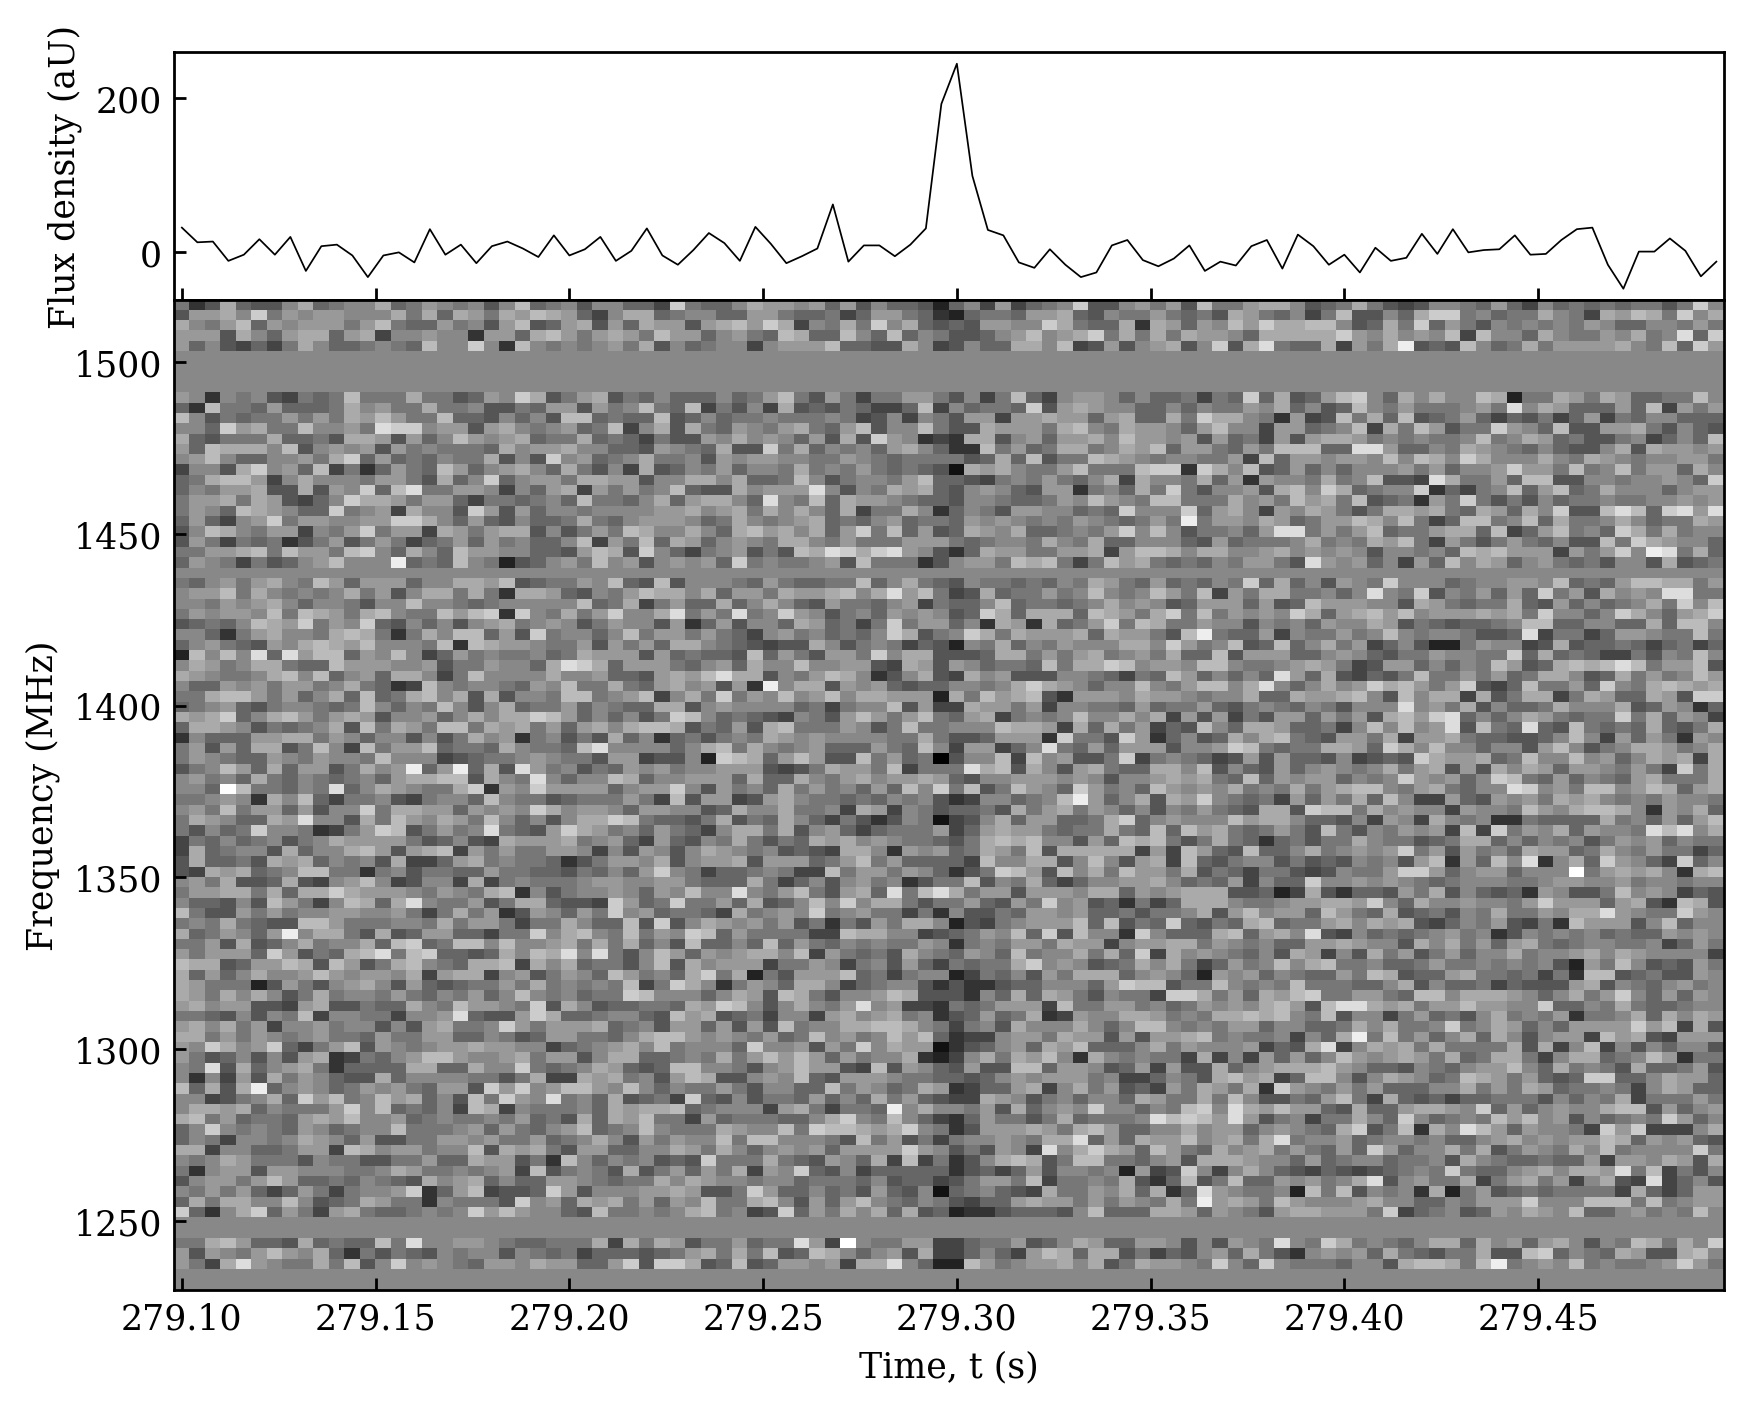
\includegraphics[width=0.8\textwidth]{Images/FRB010621dedisp.jpg}
    \caption[Dedispersion]{Frequency spectrum and pulse profile for data from FRB 010621 before (upper) and after (lower) dedispersion at 748$\cmp$.}
    \label{fig:dedisp}
\end{figure}

The second operation is the boxcar matched filter. This process searches for burst signals in the dedispersed time series using a matched filter. Here it is assumed that the FRB can be approximated by a square wave shape, hidden in Gaussian noise. The template of the filter for an FRB with amplitude, pulse center and width of $A$, $t_0$, and W respectively, is given by
\begin{equation} \label{eq:filter}
    h(t,t_0,W) = \begin{cases}A, &\text{ if } \left|t-t_0\right| \leq W/2, \\
    0, &\text{ otherwise}\end{cases}
\end{equation}
The concept that is used here to find the burst is called the likelihood ratio test, quoted as the `most powerful test' \cite{fisz1963probability}. The key is the detection statistic $S$ defined as the logarithmic likelihood ratio between the cases of having and not having the signal i.e.
\begin{equation}\label{eq:stat}
    S \equiv \frac{\Lambda_{\text{Sig}}}{\Lambda_{\text{Null}}} = \frac{\mathbf{s}^2 - (\mathbf{s}-\mathbf{h})^2}{2\sigma^2}
\end{equation}
where $\sigma$ is the standard deviation of the noise present, assuming it is Gaussian noise. With the filter established in Equation \ref{eq:filter}, Equation \ref{eq:stat} reduces to 
\begin{equation}\label{eq:s}
    S = \frac{1}{N_{\text{box}}\sigma^2} \left(\sum_{\left|t-t_0\right|\leq W/2} s(t)\right)^2
\end{equation}
where $N_{\text{box}}$ is the number of data points in the burst. This is directly related to the SNR of the burst i.e. $\text{SNR} = \sqrt{S}$. 

To perform this, the boxcar filter is produced for a certain pulse width and is convolved with a time series at a certain DM. Convolution is defined as an integral that expresses the amount of overlap of two functions as they are shifted over each other i.e.
\begin{equation}
    (f*g)(t) = \int_{-\infty}^{\infty} f(t)g(t-\tau)\,d\tau
\end{equation}
In this case, both $s(t)$ and $h(t)$ are discrete, allowing the integral to be changed into a summation at all $t_0$,
\begin{equation}
    (s*h)(t_0) = \sum_{t = -\infty}^{\infty} s(t_0)h(t_0-t)
\end{equation}
which would produce the summation term in Equation \ref{eq:s} at all $t_0$ in the data.

Here, \texttt{numpy.convolve} is used to perform convolution. This produces a 1-D array of $S$ values for all possible pulse epoch in the data. Extending this to different pulse widths and time series at different DMs gives a 3-D array of $S$ at for different $t_0$, DM and W, which is referred to as an S-cube. 

%Convolution uses integrals which can be more effective than usual range checking and summation, allowing us to use much more complicated filters. E.g. exponential decay in peak due to scattering $\tau \propto \nu^{-4}$ (Petroff et al., 2019).

The final step in the analysis is to perform a peak search and clustering of candidates in the S-cube, based on \citeNP{Pang2018}. Peaks in the S-cube which are more than a certain threshold, $\gamma_0$ (usually $\gamma_0 \approx 42$) denotes an FRB candidate detection at a certain $t_0$, DM and W. To apply this, the program starts by searching for the maximum in the S-cube. If it is larger than the threshold, the program performs a neighbor search. The neighbour search inspects a region around the peak; if it matches that of a monotonically decreasing function, they are removed from the search. This is done so that other bright candidates near the peak are not shadowed. Then, the neighbours of the removed region are checked as well, until the values are lower than the threshold. This ensures the suppression of duplicate candidates. The peak is then reported as a candidate, and the search continues until all the remaining values are lower than the threshold. 

Note that for a threshold of $\gamma_0$, there is a non-zero false alarm probability i.e. false detection due to statistical fluctuation. For pure Gaussian noise, the false alarm probability is given by \cite{Men2019}
\begin{equation}
    P_{\text{FA}} = \text{erfc}\left(\sqrt{\frac{\gamma_0}{2}}\right) \simeq \sqrt{\frac{2}{\pi\gamma_0}} e^{-\gamma_0/2}
\end{equation}

\section{Output}

The final section deals with the output. There are 4 types of outputs:
\begin{itemize}
    \item Main analysis plot: A complete summary plot similar to that of the original BEAR as shown in Figure \ref{fig:main}. Consists of a waterfall data plot, S-cube colourmesh plots (DM vs t, W vs DM), S-cube plots (vs t, W, DM), highlights of the candidates (position in S-cube and in waterfall plot), and the pulse profile as well as the frequency profile of the best candidate i.e. maximum of the S-cube.
    \begin{figure}
        \centering
        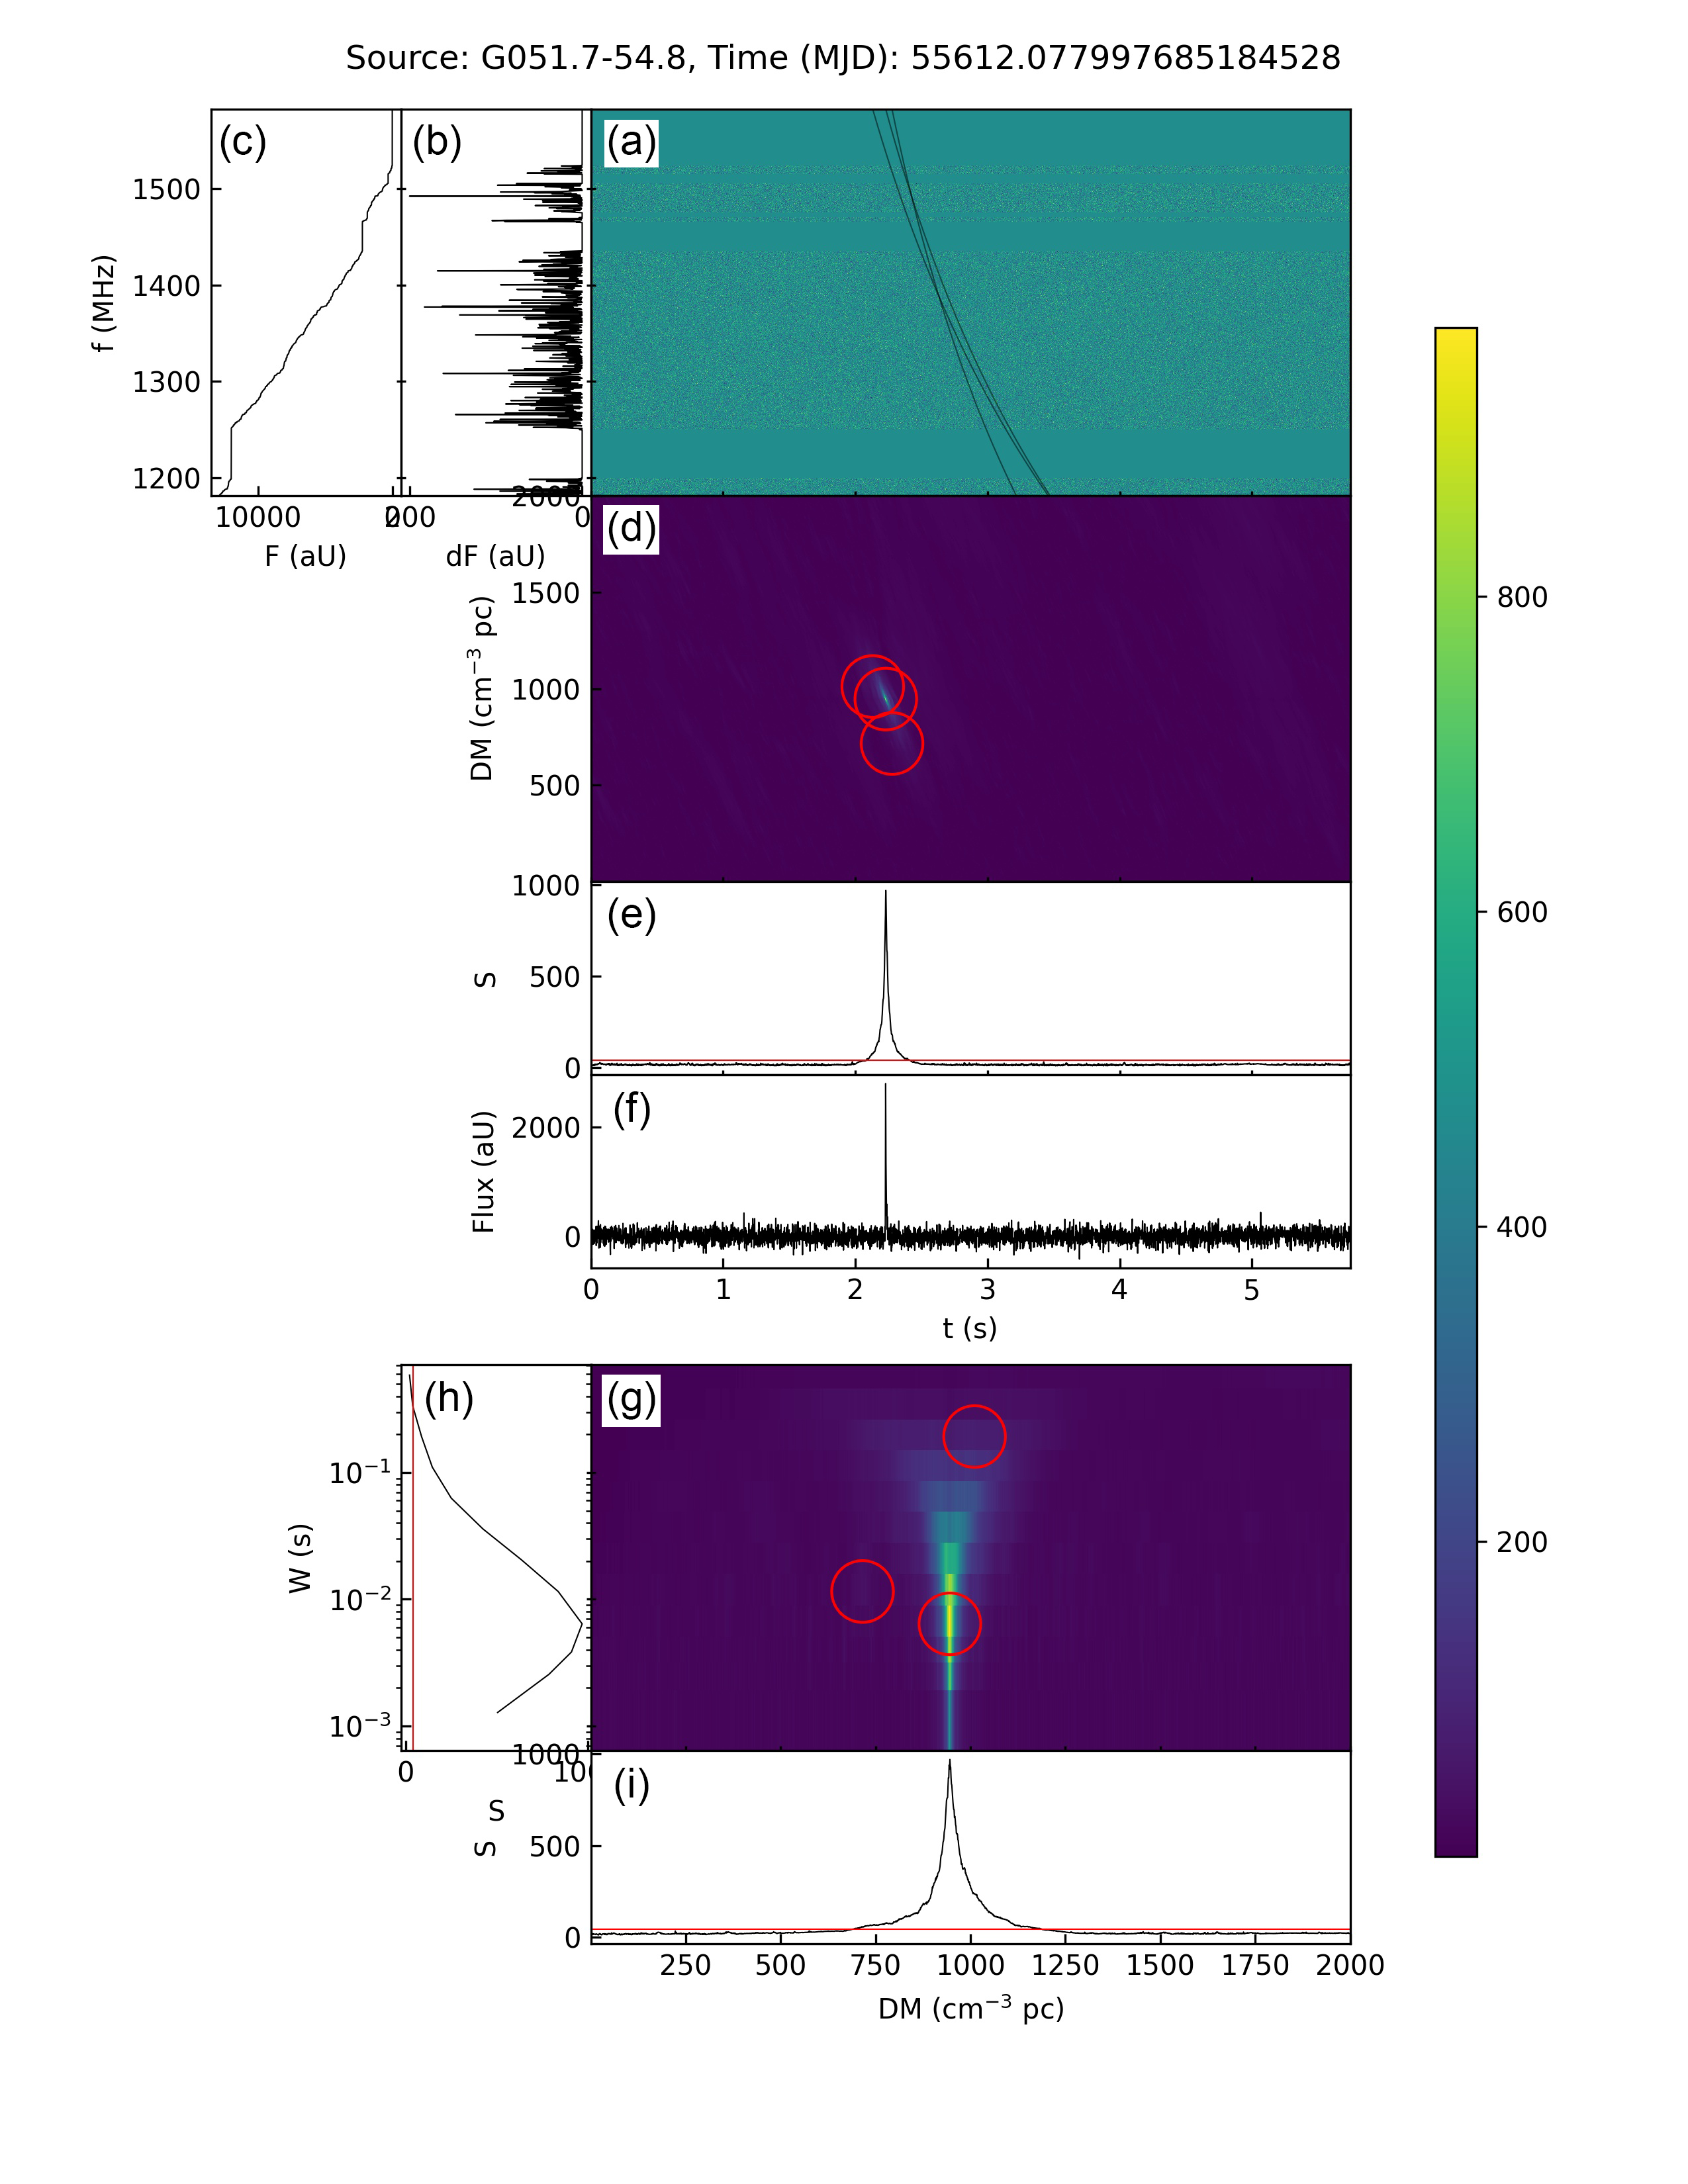
\includegraphics[width=\textwidth]{Images/Example/main.png}
        \caption[Example PoLaR BEAR main analysis plot]{Example PoLaR BEAR main analysis plot for FRB 110220. Consists of (a) filterbank data, (b) frequency profile of first candidate, (c) integrated frequency profile of first candidate, (d) S as a function of DM and time, (e) S as a function time, (f) pulse profile of first candidate, (g) S as a function of W and DM, (h) S as a function of W, and (i) S as a function of DM.}
        \label{fig:main}
    \end{figure}
    \item Candidates' pulse profile plots: Plots of the dedispersed time series at DMs of the candidates as shown in Figure \ref{fig:prof}. 
    \begin{figure}
        \centering
        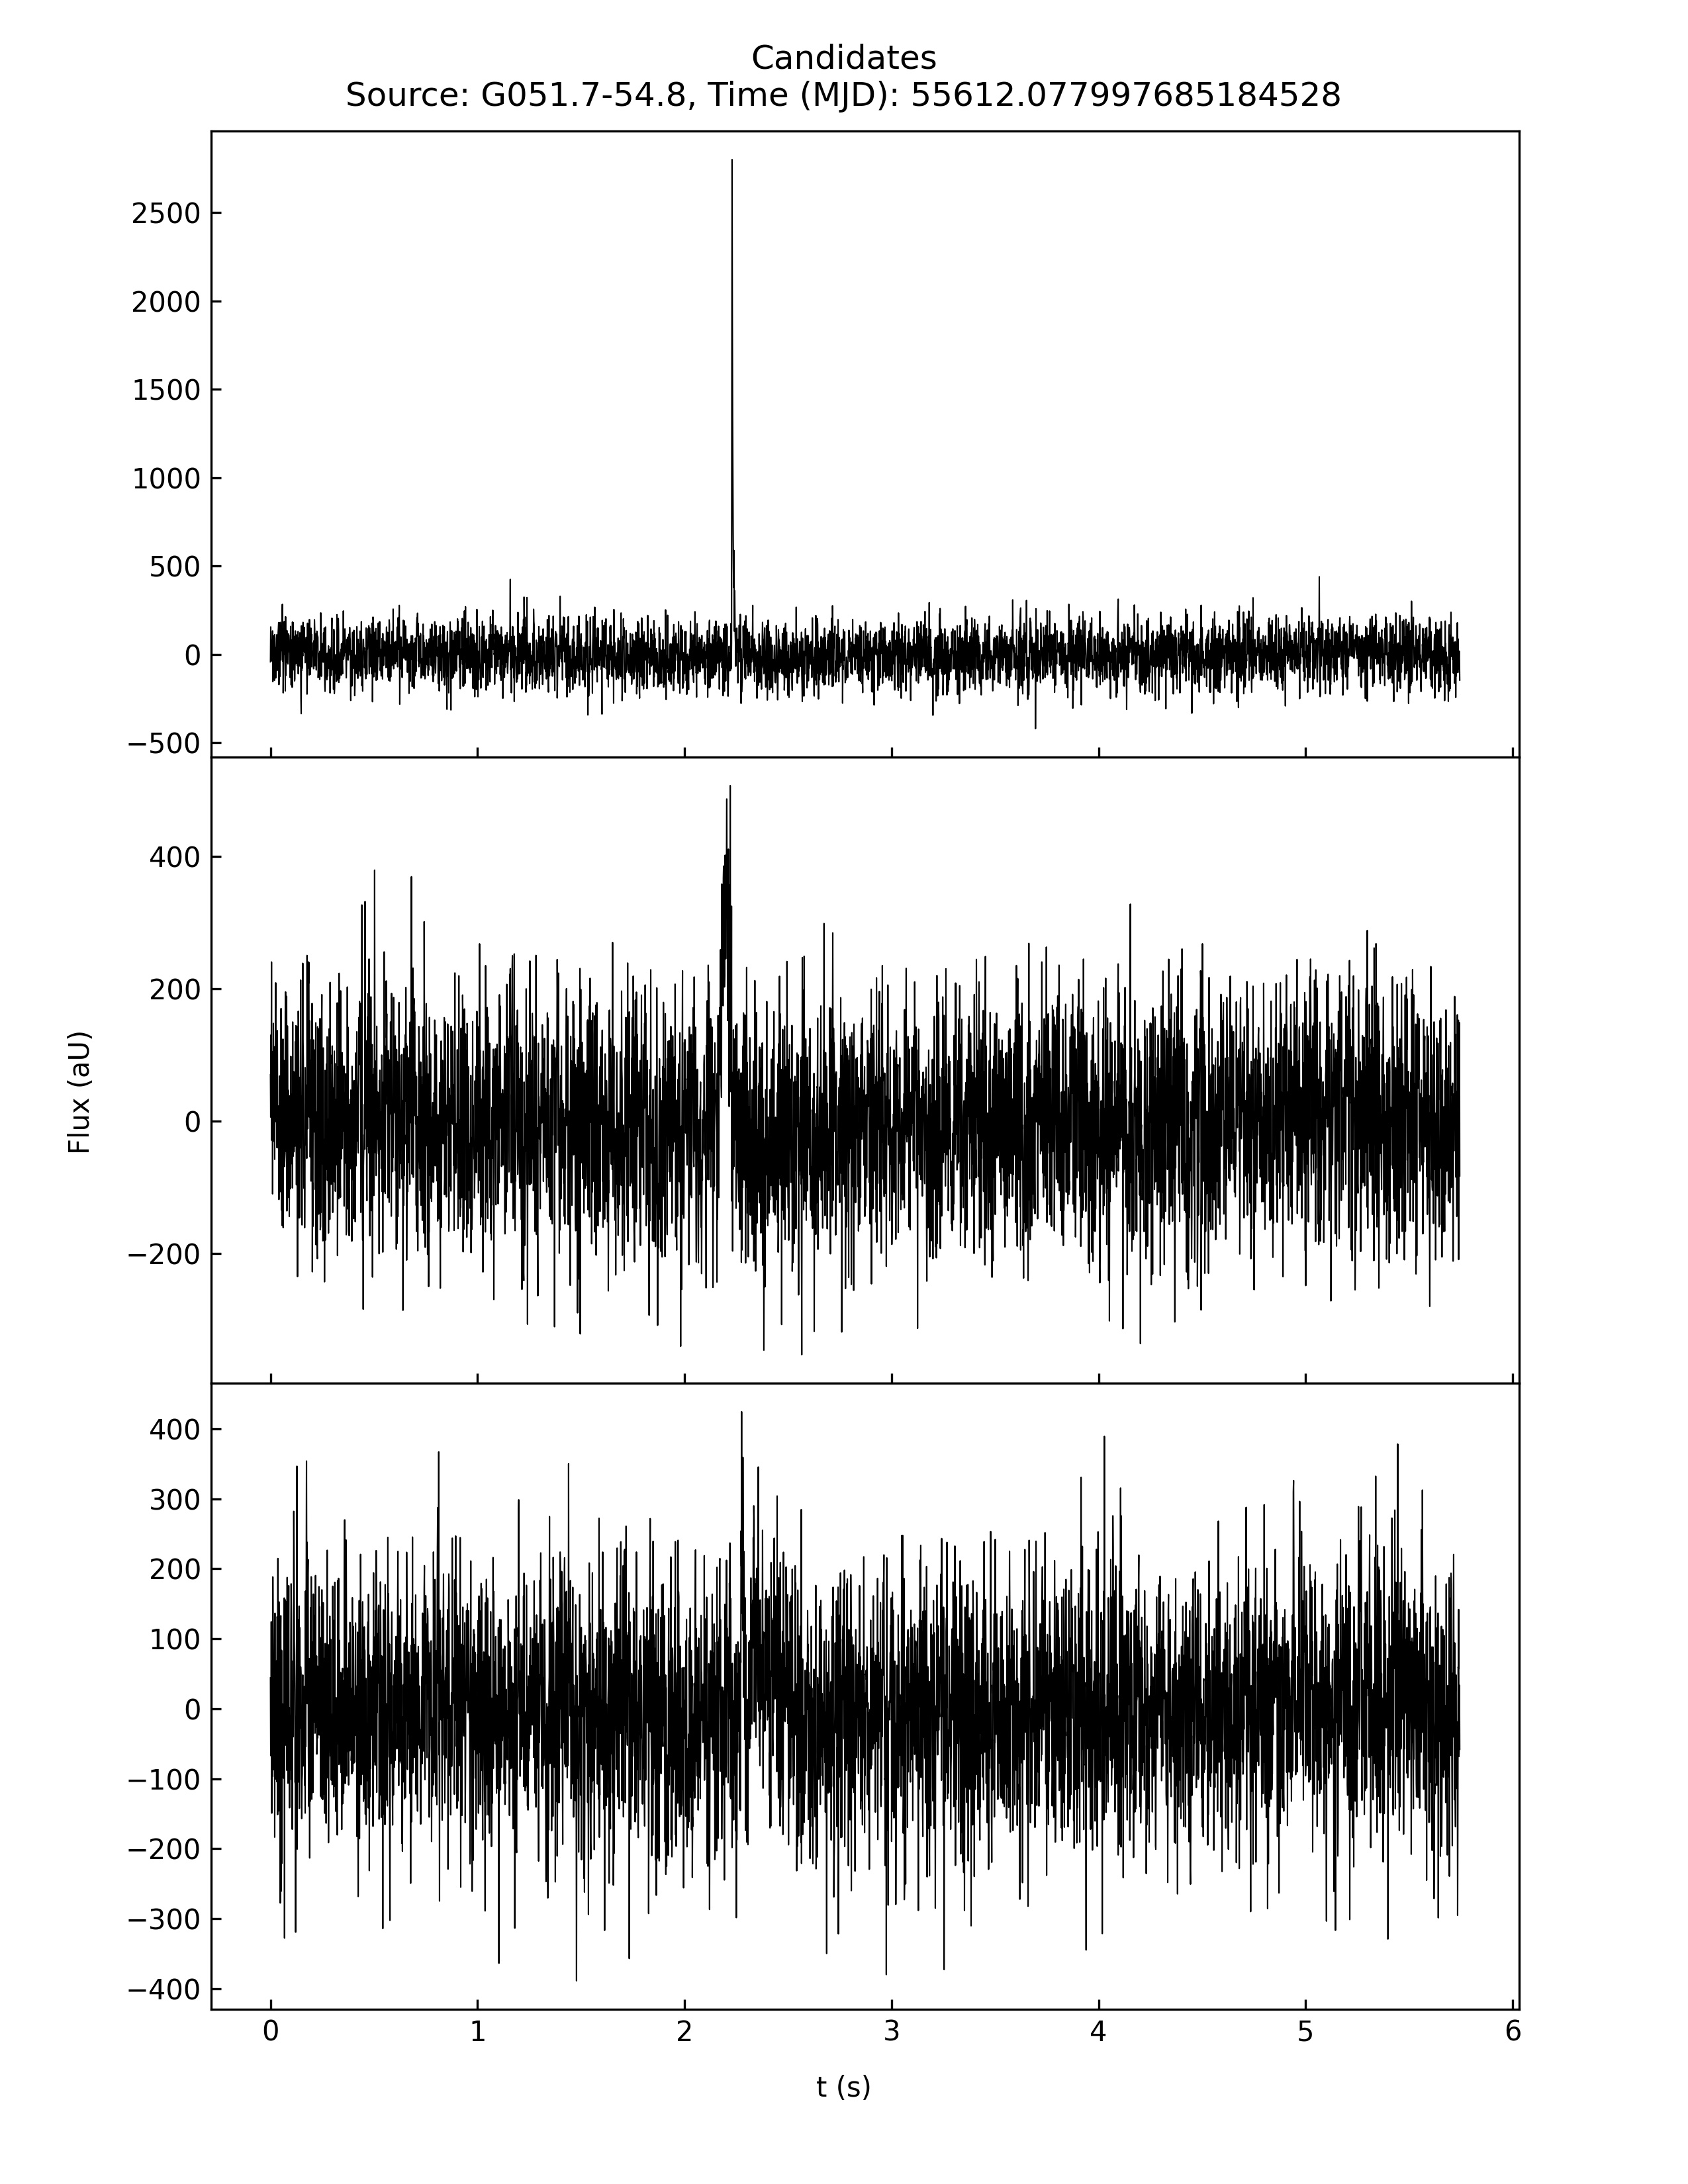
\includegraphics[width=\textwidth]{Images/Example/profile.jpeg}
        \caption[Example PoLaR BEAR candidates' pulse profile plots]{Example PoLaR BEAR candidates' pulse profile plots for FRB 110220.}
        \label{fig:prof}
    \end{figure}
    \item Candidates' analysis plots: Detailed plots of each candidates' analysis as shown in Figure \ref{fig:cand}. Detailed plots of each candidates' analysis. Consists of the pulse profile, dedispersed waterfall plot, frequency profile, localized S-cube colourmesh plots (DM vs t, W vs DM) and S-cube plots (vs W, DM).
    \begin{sidewaysfigure}
        \centering
        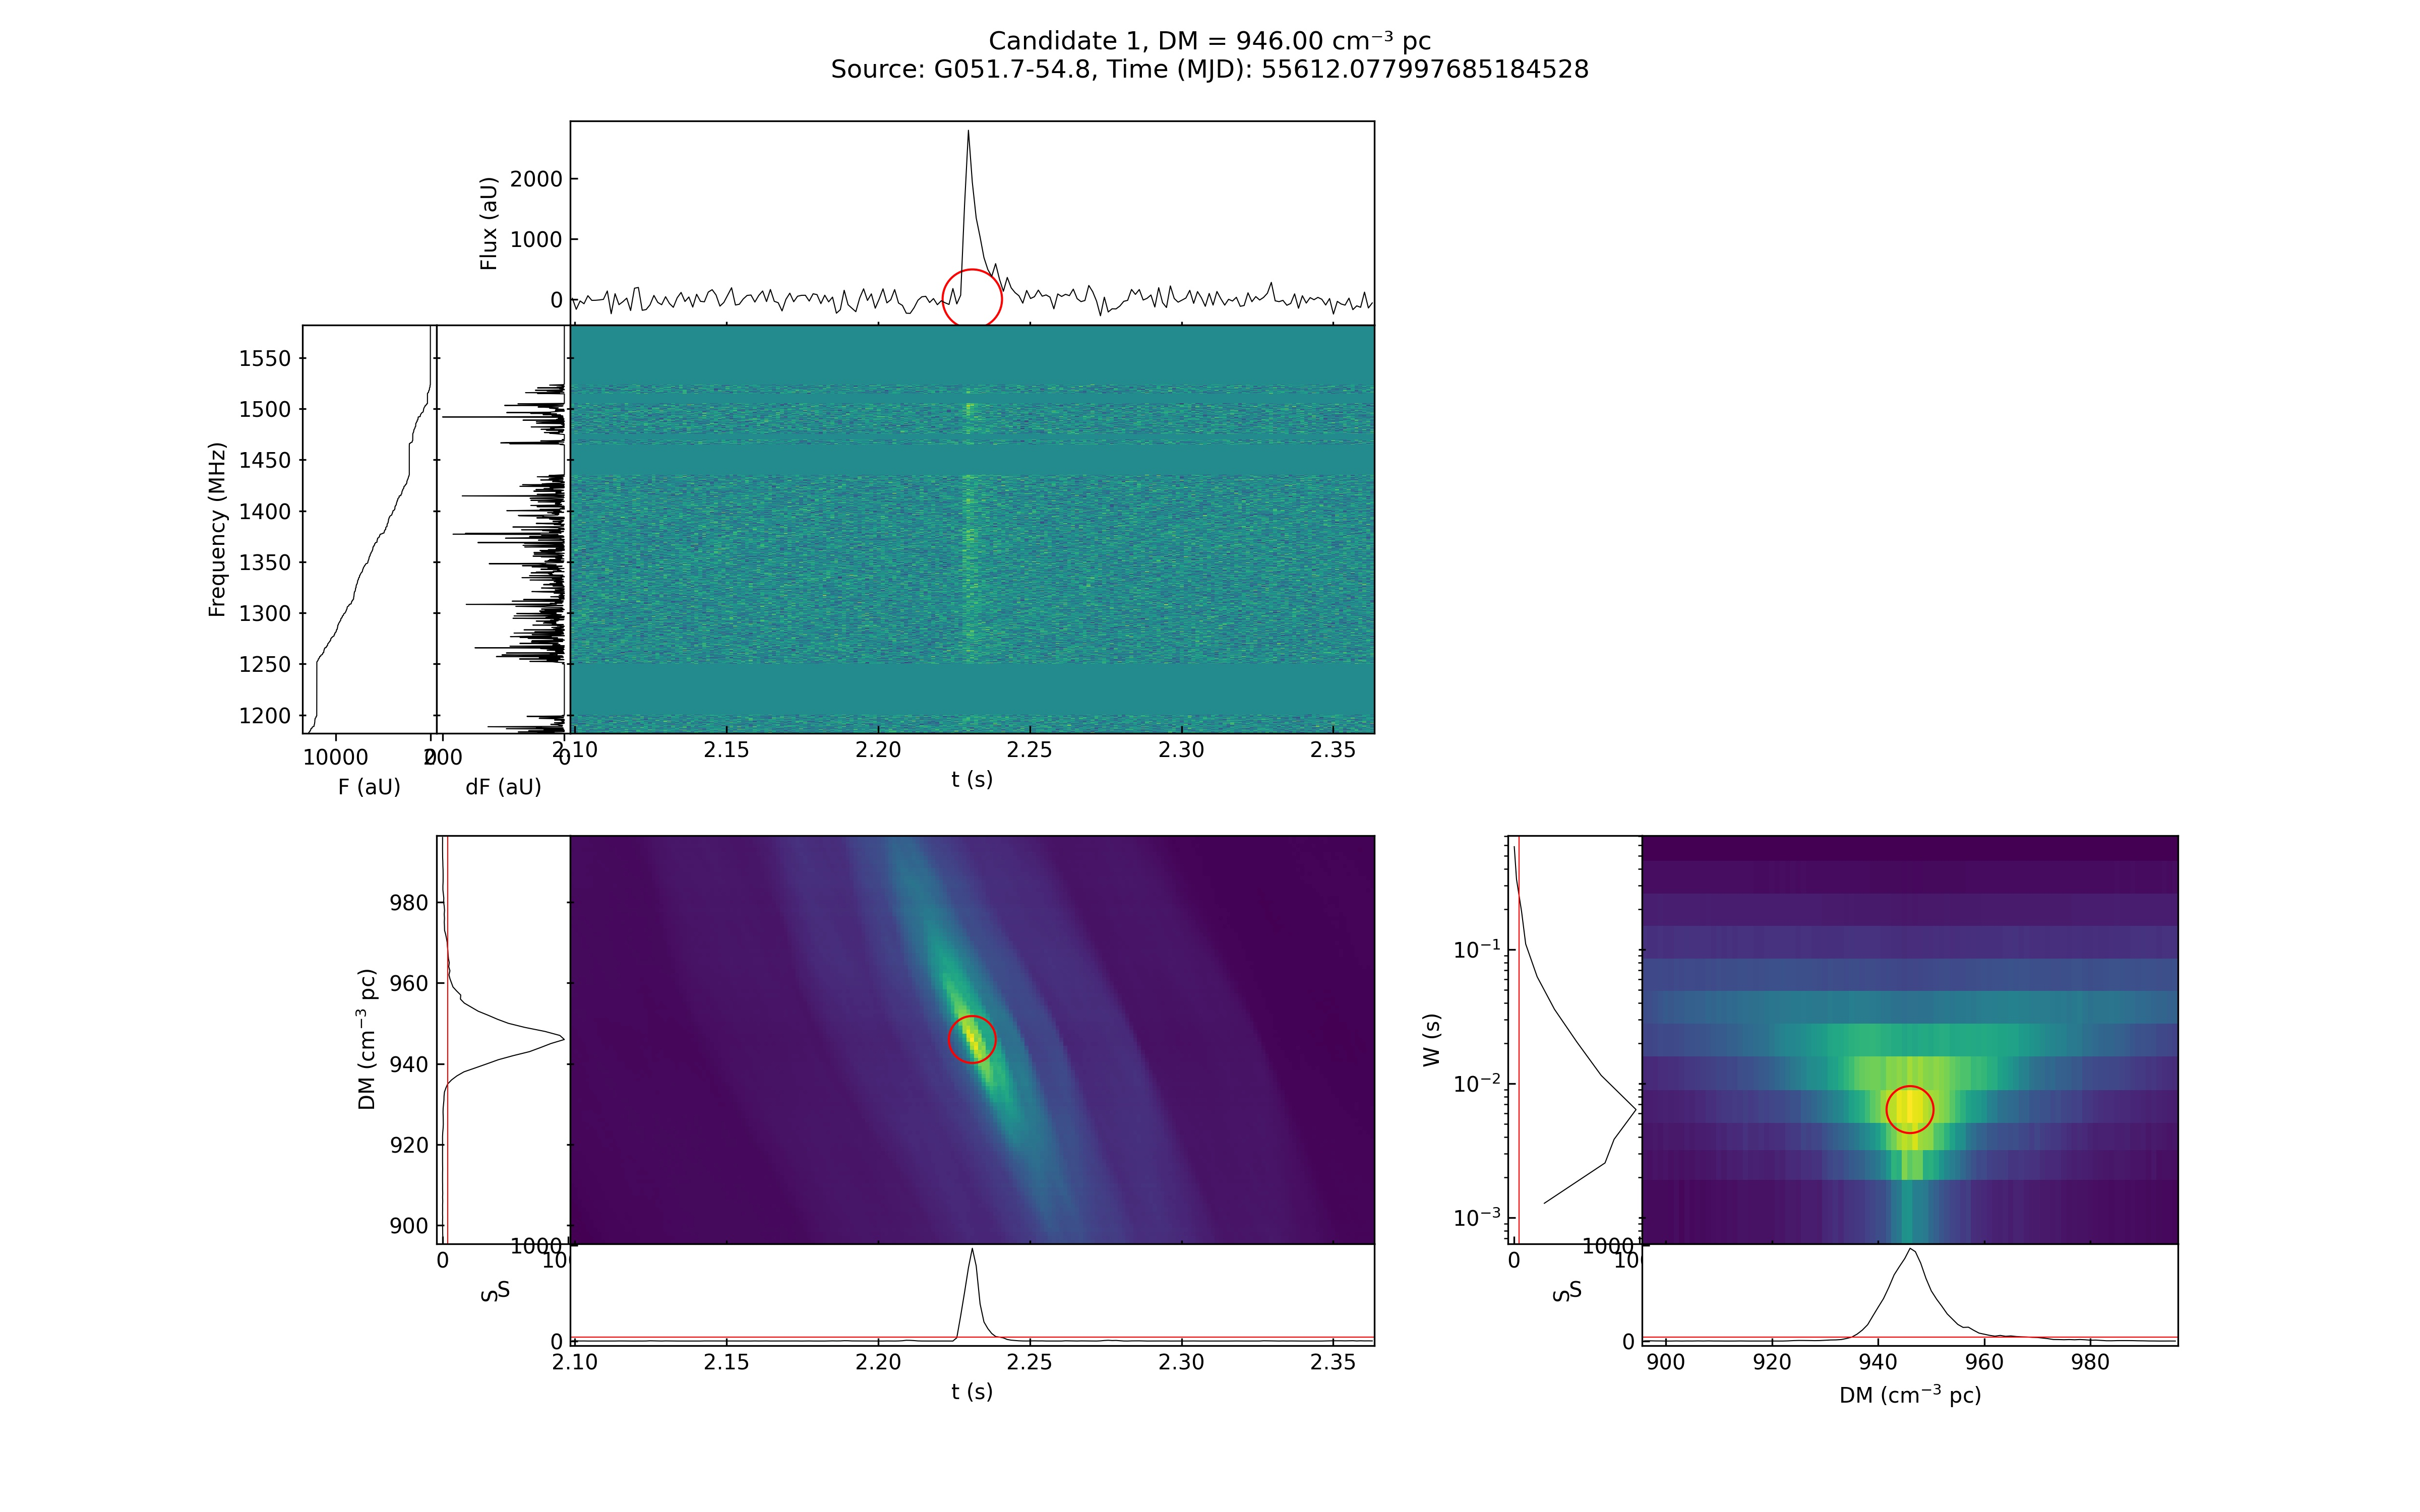
\includegraphics[width=0.9\textwidth]{Images/Example/cand.jpeg}
        \caption[Example PoLaR BEAR candidates' analysis plot]{Example PoLaR BEAR candidates' analysis plot for FRB 110220. Consists of (a) pulse profile of the candidate, (b) dedispersed filterbank data, (c) frequency profile of the candidate, (d) integrated frequency profile of the candidate, (e) S as a function of DM and time, (f) S as function of DM, (g) S as a function of time, (h) S as a function of W and DM, (i) S as a function of W, and (j) S as a function of DM.}
        \label{fig:cand}
    \end{sidewaysfigure}
    \item Analysis properties and results: A text file of the analysis parameters used and the properties of the candidates as shown in Figure \ref{fig:prop}. 
    \begin{figure}
        \centering
        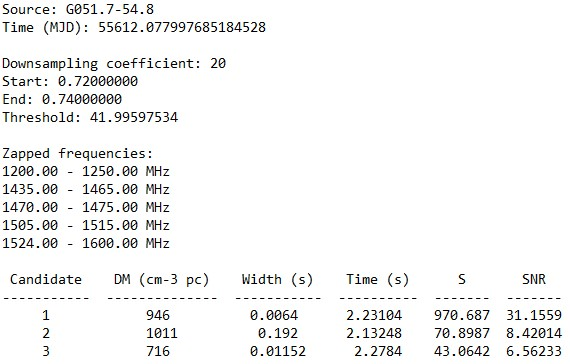
\includegraphics[width=\textwidth]{Images/Example/prop.jpg}
        \caption[Example PoLaR BEAR analysis properties and results]{Example PoLaR BEAR analysis properties and results for FRB 110220. Includes the source name, start time of the data in MJD, downsampling coefficient, start and end percentage, threshold for S, zapped frequency range, and the candidates' properties e.g., DM, width, pulse time, S, and SNR.}
        \label{fig:prop}
    \end{figure}
\end{itemize}
The plots are handled using \texttt{matplotlib.pyplot}'s functions, specifically \texttt{subplots}, \texttt{plot}, \texttt{scatter}, and \texttt{pcolormesh}, whereas the analysis properties and results text are formatted using \texttt{tabulate}. % See Appendix \ref{app:polarbear} for example outputs.
\pagebreak

\section{PoLaR BEAR Tests}

To test PoLaR BEAR, two types of data are used; real FRB data and generated FRB data. The FRB properties obtained from PoLaR BEAR are compared with the actual measured/generated properties, as well as comparing them to the original BEAR's output. 

\subsection{Real FRB data}

Here, publicly released FRB data from various radio telescopes are used, mainly the Parkes Telescope, with some from Lovell Telescope, and STARE2, consisting of the Owens Valley Radio Observatory, Goldstone Observatory, and Delta. The properties of the FRBs used are as shown in Table \ref{tab:frbdata}. The frequency channels contaminated with RFI were inspected visually and zapped accordingly.

\begin{sidewaystable}
    \centering
    \caption[Properties of real FRB data]{Properties of the real FRB data used for PoLaR BEAR tests. The true properties are taken from TNS and FRBCAT.}
    \begin{tabular}{ccccccc}
        \hline
        Telescope       & FRB Name   & Start time (MJD)      & File name (Beam)                          & DM ($\cmp$) & W (ms) & SNR  \\
        \hline
        Parkes$^{a}$         & FRB 010124 & 51934.019976851850515 & BJ0009\_02551.fil (5)                    & 790.3       & 10.6     & 10.6 \\
        Parkes$^{a}$          & FRB 010621 & 52081.539953703701030 & PM0141\_017A1.fil (10)                    & 745         & 7        & 16.3 \\
        Parkes$^{a}$          & FRB 010724 & 52114.806423611109494 & SMC021\_00861.fil (6)                    & 375         & 20       & 100  \\
        Parkes$^{b}$         & FRB 090625 & 55007.910081018519122 & 2009-06-25-21\_50\_31.fil (6)            & 899.55      & 1.92     & 30   \\
        Parkes$^{a}$          & FRB 110220 & 55612.077997685184528 & 2011-02-20-01\_52\_19.fil (3)            & 944.38      & 6.59     & 54   \\
        Parkes$^{a}$          & FRB 110626 & 55738.896585648144537 & 2011-06-26-21\_31\_05.fil (12)            & 723         & 1.41     & 12   \\
        Parkes$^{a}$          & FRB 110703 & 55745.790069444446999 & 2011-07-03-18\_57\_42.fil (5)            & 1103.6      & 3.9      & 17   \\
        Parkes$^{a}$          & FRB 120127 & 55953.339050925926131 & 2012-01-27-08\_08\_14.fil (4)            & 553.3       & 1.21     & 13   \\
        Parkes$^{b}$          & FRB 121002 & 56202.547638888885558 & 2012-10-02-13\_08\_36.fil (12)            & 1629.18     & 5.44     & 16   \\
        Parkes$^{b}$         & FRB 130626 & 56469.620752314811398 & 2013-06-26-14\_53\_53.fil (1)            & 952.4       & 1.98     & 21   \\
        Parkes$^{b}$         & FRB 130628 & 56471.164502314815763 & 2013-06-28-03\_56\_53.fil (5)            & 469.88      & 0.64     & 29   \\
        Parkes$^{b}$         & FRB 130729 & 56502.375752314816054 & 2013-07-29-09\_01\_05.fil (10)            & 861         & 15.61    & 14   \\
        Parkes$^{c}$         & FRB 140514 & 56791.712291666663077 & 2014-05-14-17\_05\_42.fil (1)            & 561.7       & 2.816    & 16   \\
        Parkes$^{d}$          & FRB 150215 & 57068.853564814817219 & 2015-02-15-20\_29\_08.fil (13)            & 1105.6      & 2.88     & 19   \\
        Lovell$^{e}$          & FRB 121102 & 57798.871967592596775 & 57798\_73718\_J0532+3305\_000027.fil & 557         & 3        & 14   \\
        STARE2 (OVRO)$^{f}$  & FRB 200428a & 58967.230011574070002 & candidate\_ovro\_20200428.fil        & 332.702     & 0.61     & 21   \\
        STARE2 (GDSCC)$^{f}$ & FRB 200428b & 58967.300127314819999 & candidate\_gdscc\_20200428.fil       & 332.702     & 0.61     & 15   \\
        STARE2 (Delta)$^{f}$ & FRB 200428c & 58967.237430555560000 & candidate\_delta\_20200428.fil       & 332.702     & 0.61     & 20  \\
        \hline
        \end{tabular}
    \footnotesize{
    \begin{tabular}{l}
        \\
        $^{a}$: \url{https://data-portal.hpc.swin.edu.au/dataset/parkes-frbs-archival-data} \\
        $^{b}$: \url{https://data-portal.hpc.swin.edu.au/dataset/fast-radio-burst-data-high-time-resolution-universe-survey-high-latitude} \\
        $^{c}$: \url{https://data-portal.hpc.swin.edu.au/dataset/fast-radio-burst-data-frb-140514} \\
        $^{d}$: \url{https://data-portal.hpc.swin.edu.au/dataset/fast-radio-burst-data-frb-150215} \\
        $^{e}$: \url{https://zenodo.org/record/3974768#.YGWzqK8zap0} \\
        $^{f}$: \url{https://data.caltech.edu/records/1647}
    \end{tabular}}
    \label{tab:frbdata}
\end{sidewaystable}

\subsection{Generated FRB data}

Another way to test the data is by producing a simulated FRB data, or commonly known as `Fake' data. To produce the data, a simple Python code is used, based on \texttt{SIGPROC}'s Fake \cite{Lorimersigproc}, which produces fake pulsar data which are used to test pulsar detection pipelines. 

The program first randomly selects the width, SNR, and DM of the generated FRB from a set range. The SNR is scaled based on Equation \ref{eq:stat}, where the channel SNR is given by 
\begin{equation}
    \text{SNR}_i = \sqrt{\frac{N_{\text{chans}}W}{t_{\text{samp}}}}
\end{equation} 
where $N_{\text{chans}}$ is the number of frequency channels and $t_{\text{samp}}$ is the sampling time. Then, the dispersion delay is calculated using Equation \ref{eq:dmdelay}. The program then passes through all the observation time of the data. If the time (with the dispersion delay considered) is in the pulse window, the data is set to $\text{SNR}_i$. Lastly, Gaussian noise is added to the entire data using \texttt{numpy.random.normal}. The program then outputs the data as a filterbank, with corresponding parameters in the header. 

50 fake FRB data was generated, with a sampling time of 64 {\textmu}s for 30 seconds observation time, 512 frequency channels with a 1200 MHz first channel and 0.1 MHz bandwidth. The fake FRBs are generated with widths between 0.5 to 5 ms, SNR between 8 and 50, and DMs between 200 and 1900 $\cmp$. The properties of the generated fake FRBs are as shown in Table \ref{tab:fakedata}.

\begin{sidewaystable}
    \centering
    \caption[Properties of fake FRB data]{Properties of the Fake FRB data used for PoLaR BEAR tests.}
    \begin{minipage}{0.5\textheight}
    \begin{tabular}{ccccc}
        \hline
          Fake  &   File name   &  DM ($\cmp$)  &  W (ms)  &   SNR   \\
        \hline
           1       & fake\_output0.fil  &    566.158    & 3.47103  & 34.1301 \\
           2       & fake\_output1.fil  &    1476.21    & 3.97177  & 46.3679 \\
           3       & fake\_output2.fil  &    1858.64    & 2.57209  & 26.5634 \\
           4       & fake\_output3.fil  &    399.97     & 2.77513  & 10.1587 \\
           5       & fake\_output4.fil  &    573.649    & 0.710951 & 16.1083 \\
           6       & fake\_output5.fil  &    1187.42    &  3.8433  & 34.5618 \\
           7       & fake\_output6.fil  &    1028.33    & 1.66997  & 42.8729 \\
           8       & fake\_output7.fil  &    1337.1     & 3.16891  & 45.5356 \\
           9       & fake\_output8.fil  &    1364.17    & 2.16554  & 15.2655 \\
          10       & fake\_output9.fil  &    1321.39    & 4.92548  & 33.4504 \\
          11       & fake\_output10.fil &    1666.28    & 3.77166  & 44.4121 \\
          12       & fake\_output11.fil &    728.46     & 2.61624  & 20.7568 \\
          13       & fake\_output12.fil &    789.509    & 1.77699  & 44.6985 \\
          14       & fake\_output13.fil &    1744.95    & 4.58435  & 37.8006 \\
          15       & fake\_output14.fil &    1530.5     & 1.14656  & 47.1532 \\
          16       & fake\_output15.fil &    742.392    & 3.77817  & 26.9581 \\
          17       & fake\_output16.fil &    1504.54    & 3.39606  & 9.8772  \\
          18       & fake\_output17.fil &    669.927    & 2.79792  & 11.7874 \\
          19       & fake\_output18.fil &    1287.46    & 1.60874  & 9.00864 \\
          20       & fake\_output19.fil &    669.849    & 3.16439  & 23.6871 \\
          21       & fake\_output20.fil &    1395.44    & 4.48013  & 39.7673 \\
          22       & fake\_output21.fil &    678.089    & 2.73084  & 21.4789 \\
          23       & fake\_output22.fil &    393.089    & 2.40809  & 35.0218 \\
          24       & fake\_output23.fil &    848.94     &  2.227   & 17.862  \\
          25       & fake\_output24.fil &    846.969    & 1.62728  & 33.0218 \\
          \hline
    \end{tabular}
    \end{minipage}%
    \begin{minipage}{0.5\textheight}
    \begin{tabular}{ccccc}
        \hline
          Fake  &   File name   &  DM ($\cmp$)  &  W (ms)  &   SNR   \\
        \hline
          26       & fake\_output25.fil &    1358.91    & 4.79527  & 18.5694 \\
          27       & fake\_output26.fil &    480.351    & 2.97478  & 42.4061 \\
          28       & fake\_output27.fil &    1668.8     & 2.42997  & 29.9655 \\
          29       & fake\_output28.fil &    359.856    &  4.1512  & 31.7901 \\
          30       & fake\_output29.fil &    426.874    & 1.36033  & 28.9338 \\
          31       & fake\_output30.fil &    1308.65    & 2.71006  & 11.783  \\
          32       & fake\_output31.fil &    352.708    & 0.863634 & 28.142  \\
          33       & fake\_output32.fil &    745.125    & 0.82552  & 32.431  \\
          34       & fake\_output33.fil &    1355.43    & 2.69499  & 34.6861 \\
          35       & fake\_output34.fil &    741.125    & 2.97293  & 11.9684 \\
          36       & fake\_output35.fil &    1046.19    & 3.98829  & 18.2477 \\
          37       & fake\_output36.fil &    1199.7     &  1.4724  & 17.7535 \\
          38       & fake\_output37.fil &    518.282    & 4.72503  & 49.626  \\
          39       & fake\_output38.fil &    1799.01    & 4.07805  & 23.5333 \\
          40       & fake\_output39.fil &    670.819    & 2.36506  & 19.3561 \\
          41       & fake\_output40.fil &    1688.62    & 0.997483 & 40.5665 \\
          42       & fake\_output41.fil &    1195.6     & 1.85354  & 30.0239 \\
          43       & fake\_output42.fil &    1869.7     & 1.82071  & 24.1694 \\
          44       & fake\_output43.fil &    587.108    & 3.61604  & 11.8553 \\
          45       & fake\_output44.fil &    601.626    & 4.16235  & 33.3841 \\
          46       & fake\_output45.fil &    746.818    & 2.50385  & 9.14934 \\
          47       & fake\_output46.fil &    1268.11    & 1.02883  & 15.4958 \\
          48       & fake\_output47.fil &    1818.44    & 4.73783  & 40.2606 \\
          49       & fake\_output48.fil &    1734.89    &  2.3775  & 40.4545 \\
          50       & fake\_output49.fil &    917.338    & 3.38351  & 40.1697 \\
        \hline
    \end{tabular}
    \end{minipage}
    \label{tab:fakedata}
\end{sidewaystable}